\documentclass[11pt,a4paper]{article}
%\pdfoutput=1
\usepackage{jheppub}
\usepackage[notref,color,draft]{showkeys}
%\usepackage[pageref]{backref}
\usepackage{amsthm,amsbsy,amsfonts,mathrsfs,enumerate,float,wrapfig,amsmath}
\usepackage{subfigure}
%\usepackage[usenames, dvipsnames]{color}
\newcommand{\nn}{\nonumber}
\newcommand{\ssk}[1]{{\color{blue}(\textbf{SSK: {#1}})}}
\newcommand{\bF}{\mathbf{F}}
\newcommand{\bS}{\mathbf{S}}
\newcommand{\AS}{\mathbf{AS}}
% \definecolor{refkey}{gray}{.55}
% \definecolor{labelkey}{gray}{.75}

%=================================================================
\title{Blow-up}
%=================================================================

\abstract{
TO DO LIST:\\
1.
}



%=================================================================
%=================================================================
\begin{document}
\preprint{
\begin{flushright}
\tt 
%preprint number
%KIAS-P*****\\
\end{flushright}
}
\today 
%\maketitle
\section{Prepotential}
The effective prepotential on a Coulomb branch of a 5d gauge theory with a gauge group $G$ and matter $f$ in a representation $R_f$ is given by [Seiberg] %\cite{Seiberg:1996bd, Morrison:1996xf, Intriligator:1997pq}\footnote{In \cite{Closset:2018bjz}, the authors approach the prepotential differently.}
\begin{align}
\mathcal{F}(\phi) = \frac{m_0}{2}h_{ij}\phi_i\phi_j + \frac{\kappa}{6}d_{ijk}\phi_i\phi_j\phi_k + \frac{1}{12}\left(\sum_{r\in\text{roots}}\left|r\cdot \phi\right|^3 - \sum_f\sum_{w \in R_f}\left|w\cdot \phi - m_f\right|^3\right). \label{prepotential}
\end{align}
Here, $m_0$ is the inverse of the squared gauge coupling, $\kappa$ is the classical Chern-Simons level and $m_f$ is a mass parameter for the matter $f$. $r$ is a root of the Lie algebra $\mathfrak{g}$ associated to $G$ and $w$ is a weight of the representation $R_f$ of $\mathfrak{g}$. We also defined $h_{ij} = \text{Tr}(T_iT_j), d_{ijk} = \frac{1}{2}\text{Tr}\left(T_i\{T_j, T_k\}\right)$ where $T_i$ are the Cartan generators of the Lie algebra $\mathfrak{g}$.
\subsection{$SU(6)_\kappa+1{\bf TAS}$}
The prepotential for $SU(6)_\kappa+1{\bf TAS}$ is written as 
\begin{align}
\mathcal{F}^{SU(6)_{\kappa}}_{N_{{\bf TAS}}=1} = \frac{m_0}{2}\sum_{i=1}^6a_i^2 + \frac{\kappa}{6}\sum_{i=1}^6a_i^3 +\frac{1}{6}\bigg(\sum_{1 \leq i < j \leq 6}(a_i - a_j)^3 - \sum_{2 \leq i < j \leq 6}(a_1 + a_i + a_j)^3\bigg), \label{eq:preSU6TSA}
\end{align}
where $\kappa$ is the CS level. 

Now we choose $\kappa=3$. In Dynkin basis, one can re-express the prepotential for $SU(6)_3+1{\bf TAS}$, using the relation
\begin{align}
	a_1= \phi_1,&& 
	a_2=\phi_2-\phi_1,&&
	a_3=\phi_3-\phi_2,&&
	a_4=\phi_4-\phi_3,&&
	a_5=\phi_5-\phi_4,&&
	a_6=-\phi_5, \label{orth2Dynkin}
\end{align}
as follows:
\begin{align}
	\mathcal{F}=&\,m_0 \big( \phi _1^2-\phi _2 \phi _1+\phi _2^2+\phi _3^2+\phi _4^2+\phi _5^2-\phi _2 \phi _3-\phi _3 \phi _4-\phi _4
   \phi _5\big) \cr
   &+ \frac{\phi _1^3}{3}+4 \phi _2 \phi _1^2-5 \phi _2^2 \phi _1+2 \phi _2 \phi _3 \phi _1-2 \left(\phi
   _3^2-\phi _4 \phi _3+\phi _4^2+\phi _5^2-\phi _4 \phi _5\right) \phi _1\cr
  & +\frac{4 \phi _2^3}{3}+\frac{4
   \phi _3^3}{3}+\frac{4 \phi _4^3}{3}+\frac{4 \phi _5^3}{3}-2 \phi _2 \phi _3^2-\phi _3 \phi _4^2+\phi
   _2^2 \phi _3-\phi _4^2 \phi _5. \label{eq:prep+SU6-3}
\end{align}
One can obtain the monopole string tensions $T_i$ from this prepotential. 
%%%%%%%%%%%%%
\subsection{5-brane web configuration}
It follows from [arXiv:1902.04754]  that a 5-brane web diagram for $SU(6)_3+1{\bf TAS}$ is depicted in Figure \ref{fig:SU6-monopole}.
%---------  Figure  ---------------%
\begin{figure}[t]
\centering
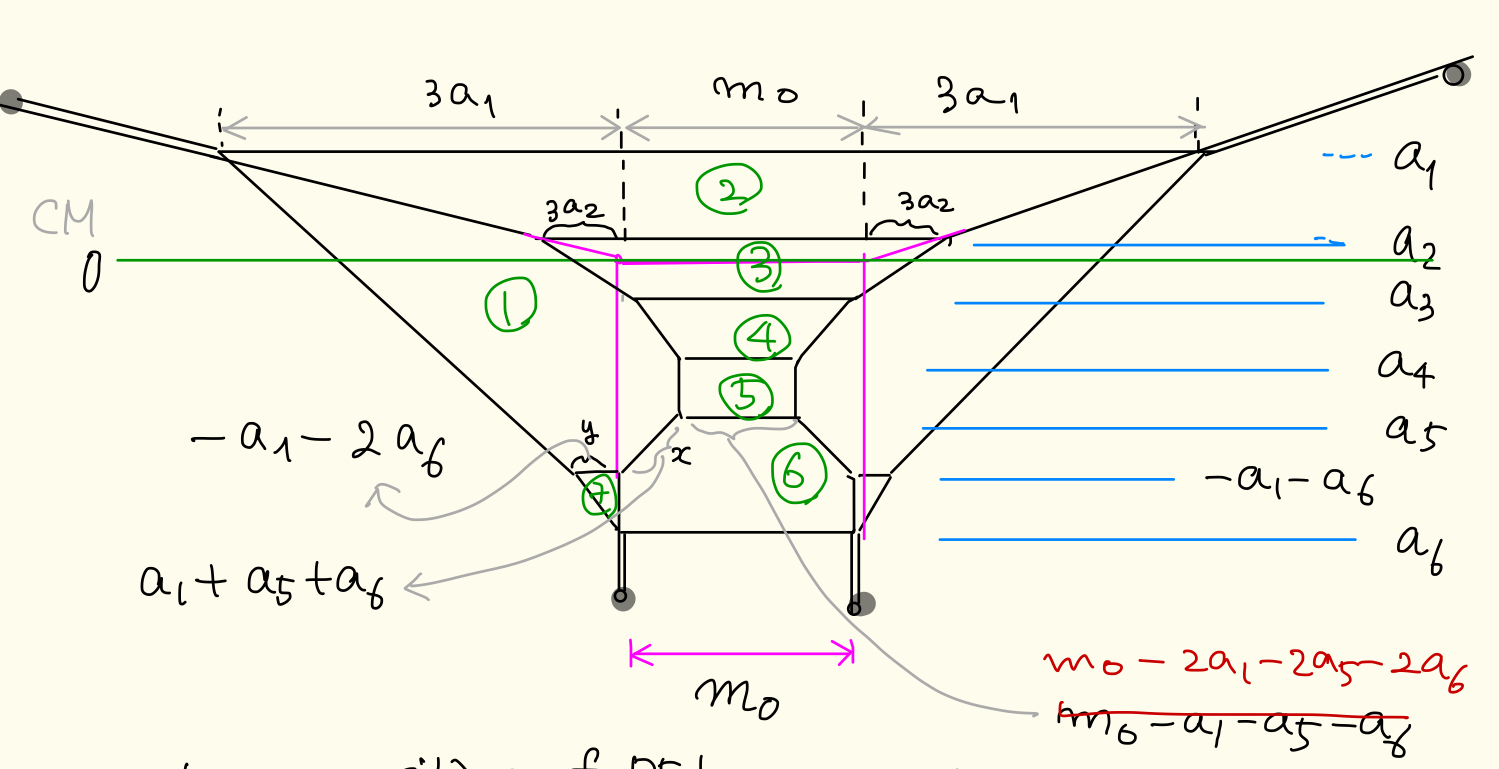
\includegraphics[width=10cm]{SU6-monopole.jpeg}
\caption{A 5-brane web for $SU(6)_3+1{\bf TAS}$ with massless ${\bf TAS}$.}
\label{fig:SU6-monopole}
\end{figure}
%----------------------------------%
It is straightforward to see that the area of the faces in the web diagram agrees with the monopole string tensions $T_i$ from the prepotential \eqref{eq:prep+SU6-3}:
\begin{align}
T_1=\textcircled{\scriptsize 1} + 2\textcircled{\scriptsize 2},  %\crcr
&& T_2=\textcircled{\scriptsize 3}, %\crcr
&&T_3=\textcircled{\scriptsize 4}, %\crcr
&&T_4=\textcircled{\scriptsize 5}, %\crcr
&&T_5=\textcircled{\scriptsize 6} 
	+ 2\textcircled{\scriptsize 7},
\end{align}
where the encircled numbers represent the area of apparent faces in Figure \ref{fig:SU6-monopole}.

We note that there is a special Higgs phase that the 
 $SU(6)_3+1{\bf TAS}$ can be expressed as a product of two pure $SU(3)_3$ theory. To this end, consider the following parameter relation
 \begin{align}
 	a_5= - a_1-a_6, \qquad {\rm or} \qquad \phi_4=\phi_1. \label{Higgising}
 \end{align}
 This is when the parameter $x$ becomes $0$ such that two D5-brane lined up. From usual Higgsing that branes disjoint and rejoin to other brane \ref{fig:SU6-Higgsing}(a), one expects that the web diagram configuration is that of two pure $SU(3)_3$ theory, as depicted in Figure \ref{fig:SU6-Higgsing}(b). 
  %---------  Figure  ---------------%
\begin{figure}[t]
\centering
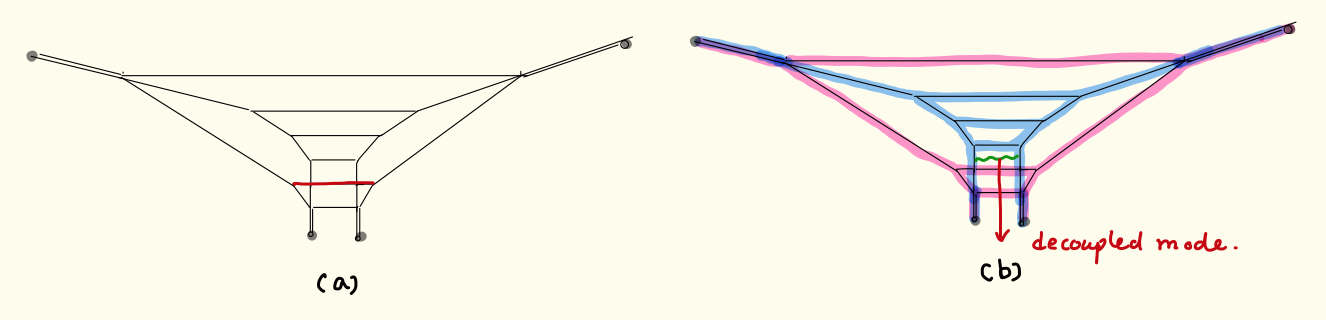
\includegraphics[width=12cm]{SU6-Higgsing.jpeg}
\caption{(a) A Higgsing from from $SU(6)_3+1{\bf TAS}$ to two $SU(3)_3$ theories. (a) Two $SU(3)_3$ theories are painted in blue and in pink respectively. A new decoupled mode emerges.}
\label{fig:SU6-Higgsing}
\end{figure}
%----------------------------------%
The prepotential with this Higgsings is indeed written as a sum of two pure $SU(3)_3$ theories.
From \ref{prepotential}, the prepotential for $SU(3)_3$ is given by
\begin{align}
\mathcal{F}_{SU(3)_{3}} (\tilde a_1,\tilde a_2,\tilde a_3)= \frac{m_0}{2}\sum_{i=1}^3\tilde a_i^2 + \frac{1}{2}\sum_{i=1}^3 \tilde a_i^3 +\frac{1}{6}\sum_{1 \leq i < j \leq 3}(\tilde a_i - \tilde a_j)^3 , 
\end{align}
where $\sum_{i=1}^3 \tilde a_i=0$. From Figure \ref{fig:SU6-Higgsing}, the Coulomb branch parameters for two $SU(3)_3$ theories read $(a_1, a_5, a_6)$ and $(a_2, a_3, a_4)$. It follows from the $SU(6)$ traceless condition $a_1+a_2+a_3+a_4+a_5+a_6=0$ before the Higgsing, these two $SU(3)$ Coulomb branch parameters automatically satisfy the $SU(3)$ traceless condition with the Higgsing \eqref{Higgising}, 
\begin{align}
	a_1+a_5+a_6=0, \qquad {\rm and} \qquad a_2+a_3+a_4=0.
\end{align}
One then readily see that 
\begin{align}
\mathcal{F}^{SU(6)_{3}}_{N_{{\bf TAS}}=1}{}\bigg|_{a_1+a_5+a_6\to0}	\rightarrow \mathcal{F}_{SU(3)_{3}} (a_1, a_5,a_6) + \mathcal{F}_{SU(3)_{3}} (a_2, a_3,a_4).
\end{align}
In terms of Dynkin label,
\begin{align}
\mathcal{F}^{SU(6)_{3}}_{N_{{\bf TAS}}=1}{}\bigg|_{\phi_4\to\phi_1}	\rightarrow \mathcal{F}_{SU(3)_{3}} (\phi_1, \phi_5-\phi_1,-\phi_5) + \mathcal{F}_{SU(3)_{3}} (\phi_2-\phi_1, \phi_3-\phi_2,\phi_1-\phi_3).
\end{align}
This Higgsing may be understood as follows. Under the embedding
\begin{align}
	SU(6) \supset SU(3) \times SU(3) \times U(1),
\end{align}
the hypermultiplet in the rank-3 antisymmetric representation and the adjoint of $SU(6)$ are decomposed as
\begin{align}
	SU(6) &\supset SU(3) \times  SU(3) \times U(1),\crcr
	{\bf 35 }& ={\bf (1,1)_0 + (1,8)_0 + (8,1)_0 + (3,\bar3)_2 +(\bar3, 3)_{-2}},\crcr
	{\bf 20}&={\bf (1,1)_3 + (1,1)_{-3}+ (3,\bar3)_{-1}+(\bar3, 3)_{1} 
	}.	
\end{align}
The fields which are charged under the $U(1)$, then get masses when the vev of the Coulomb branch modulus for the $U(1)$ is given. With large vev, the fields charged under the $U(1)$ decouple and the low energy effective theory becomes rank 2 pure $SU(3)$ theory, which is a pure $SU(3)_3\times SU(3)_3$ theory without bifundamental matter.



An immediate implication is that this Higgsing gives a consistency check for the blowup formula for $SU(6)_{3}+1{\bf TAS}$, that the partition function $Z_{SU(6)_{3}+1{\bf TAS}}$ has the Higgs phase
\begin{align}
Z_{SU(6)_{3}+1{\bf TAS}}\bigg|_{\rm Higgsing}\qquad \rightarrow\qquad Z^{(1)}_{SU(3)_{3}}Z^{(2)}_{SU(3)_{3}}\,Z^{}_{\rm decoupled}\,,	
\end{align}
where 
\begin{align}
	Z^{(1)}_{SU(3)_{3}} &= Z^{(1)}_{SU(3)_{3}} (\phi_1, \phi_5-\phi_1,-\phi_5),\crcr
	Z^{(2)}_{SU(3)_{3}} &= 	Z^{(2)}_{SU(3)_{3}}(\phi_2-\phi_1, \phi_3-\phi_2,\phi_1-\phi_3), 
\end{align}
and $Z_{\rm decoupled}$ represents the extra term that does not depend on the Coulomb branch parameters, which would correspond to a new decoupled mode shown in Figure \ref{fig:SU6-Higgsing}. 
This also means, we can see some partial information of the partition function for $SU(6)_{3}+1{\bf TAS}$, as the $Z_{SU(3)_{3}}$ partition function $Z_{SU(3)_{3}}$ can be easily computed, up to the extra term. 
%%%%%%%%%%%%%%%%%%%%%%%%%%%%%%%%%%%%%%%%
\section{$SU(6)$ theory with a full rank-3 antisymmetric hypermultiplet}

%---------  Figure  ---------------%
\begin{figure}[t]
\centering
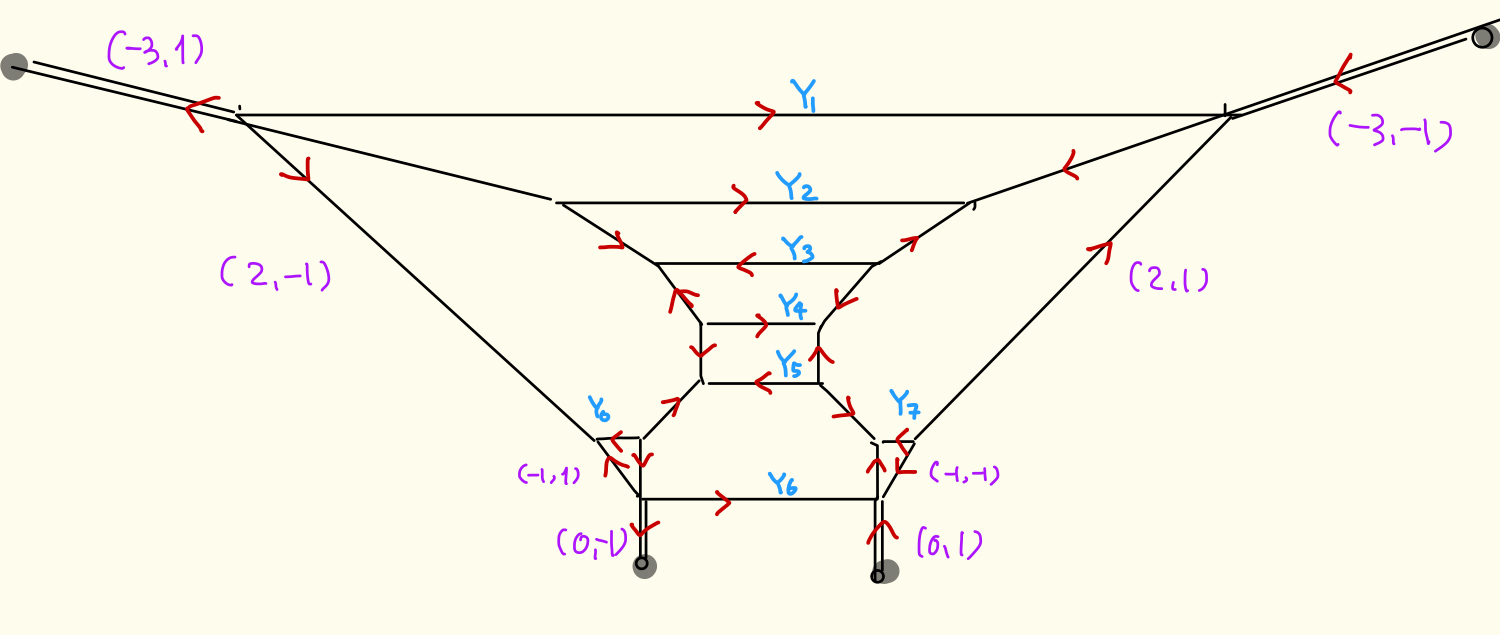
\includegraphics[width=10cm]{SU6young.jpeg}
\caption{A labeling of Young diagrams assigned to the horizontal lines in Figure \ref{fig:SU6-monopole}.}
\label{fig:SU6young}
\end{figure}
%----------------------------------%

\begin{align}
Z_{\text{Nek}} 
=&\, \sum_{\vec{Y}}q^{\sum_{i=1}^6|Y_i|} (-A_1^6)^{|Y_1|}(-A_2^6)^{|Y_2|}
%(-A_2^2A_3^2A_4^2)^{|Y_3|}(-A_2^2A_3^4)^{|Y_4| + |Y_5|}
(-A_2^2A_3^4)^{|Y_3|} (-A_2^2A_3^2A_4^2)^{|Y_4| + |Y_5|}
\nn\\
&\times f_{Y_1}(g)^5f_{Y_2}(g)^5f_{Y_3}(g)^3f_{Y_4}(g)f_{Y_5}(g)^{-1}f_{Y_6}(g)^{2}Z_{\text{left}}(\vec{Y})Z_{\text{right}}(\vec{Y}), \label{Znek1}
\end{align}
where $\vec{Y}=(Y_1, Y_2, Y_3, Y_4, Y_5, Y_6)$.
$Z_{\text{left}}(\vec{Y})$ and $Z_{\text{right}}(\vec{Y})$ are given by
\begin{align}
Z_{\text{left}}(\vec{Y})=& \,
\sum_{Y_0} ( - A_1{}^{-1} A_6{}^{-2})^{|Y_0|} 
g^{\frac{||Y_0^t||^2+||Y_0||^2}{2}} \tilde{Z}_{Y_0}^2 f_{Y_0}^2(g)
\prod_{i=1}^6 g^{\frac{||Y_i||^2}{2}} \tilde{Z}_{Y_i} 
\cr 
& 
\times 
R_{Y_1 Y_6^t}^{-1} (A_1 A_6{}^{-1})\,R_{Y_0 Y_6^t}^{-1} (A_1{}^{-1} A_6{}^{-2})\,R_{Y_1Y_0^t }^{-1} (A_1^2A_6) \cr 
& 
\times  
 \prod_{2 \le i <  j \le 5} R_{Y_i Y_j^t}^{-1} (A_i A_j{}^{-1})
 \prod_{i=2}^5 R_{Y_0^t Y_i} (A_1 A_i  A_6) ,
\end{align}
and
\begin{align}
Z_{\text{right}}(\vec{Y})=&\, Z_{\text{left}}(\vec{Y})\,/.\,\{Y_0 \to Y_7 \}~.
%{}\Big|_{Y_0\to Y_7}.
%\sum_{Y_7} ( - A_1{}^{-1} A_6{}^{-2})^{|Y_7|} 
%g^{\frac{||Y_7^t||^2+||Y_7||^2}{2}} \tilde{Z}_{Y_7}^2 f_{Y_7}^2(g)
%\prod_{i=1}^6 g^{\frac{||Y_i||^2}{2}} \tilde{Z}_{Y_i} 
%\cr 
%& 
%\times 
%R_{Y_1 Y_6^t}^{-1} (A_1 A_6{}^{-1})\,R_{Y_7 Y_6^t}^{-1} (A_1{}^{-1} A_6{}^{-2})\,R_{Y_1Y_7^t }^{-1} (A_1^2A_6) \cr 
%& 
%\times  
% \prod_{2 \le i <  j \le 5} R_{Y_i Y_j^t}^{-1} (A_i A_j{}^{-1})
% \prod_{i=2}^5 R_{Y_7^t Y_i} (A_1 A_i  A_6) .
\end{align}
Here, 
\begin{align}
A_6 
= \prod_{i=1}^5 A_i{}^{-1}, 
\quad
\tilde{Z}_{\lambda} 
= \prod_{(i,j) \in \lambda} \frac{1}{1 - g^{\lambda_i + \lambda^t_j - i - j +1} } , 
\quad
R_{\lambda \mu } (Q)= \prod_{i.j=1}^{\infty} (1 - Q g^{i+j-\lambda_j - \mu_i -1}).
\end{align}
$f_{Y}(g)$ is the framing factor defined by
\begin{align}
f_Y(g) = (-1)^{|Y|}g^{\frac{1}{2}(g^{||Y^t||^2 - ||Y||^2})},
\end{align}
%Moreover, $A_i, (i=1, \cdots, 6)$, $q$ and $g$ are defined by 
and the Coulomb branch parameters $A_i, (i=1, \cdots, 6)$, the instanton fugacity $q$ and the unrefined $\Omega$-deformation parameter $g$ are defined by 
\begin{align}
A_i = e^{-a_i}, \qquad q = e^{-m_0}, \qquad g=e^{-\epsilon}.
\end{align}

The partition function can be written as a sum of the instanton partition functions 
\begin{align}
Z_{\text{Nek}} = Z_{\text{pert}}\left(1 + \sum_{k=1}^{\infty}q^kZ_k\right) ,
\end{align}
where $Z_{\text{pert}}$ represents the perturbative part of the partition function given by the order $q^0$ in \eqref{Znek1}, while $Z_k$ stands for the $k$-instanton partition function.

\paragraph{The perturbative part.}
By setting $Y_1=Y_2=\cdots = Y_6 = \emptyset$ in  \eqref{Znek1}, the partition part is obtained 
\begin{align}
Z_{\rm pert} 
=& \,
Z_{\text{left}}( (\emptyset,\emptyset,\emptyset,\emptyset,\emptyset,\emptyset ) )
Z_{\text{right}}( (\emptyset,\emptyset,\emptyset,\emptyset,\emptyset,\emptyset ) )
\cr
=&\, 
\text{PE} \Biggl[ 
\frac{2g}{(1-g)^2} 
\Bigl( A_1 A_6{}^{-1} 
+ A_1{}^{-1} A_6{}^{-2} + A_1^2  A_6 
+ \sum_{2 \le i <  j \le 5} A_i A_j{}^{-1}
%+ \sum_{1 \le i <  j \le 6} A_i A_j{}^{-1}
%\\ 
%& \qquad \qquad \qquad \qquad 
- \sum_{i=2}^5 A_1 A_i  A_6
\Bigr)
\Biggr]
\cr 
& 
%\times \prod_{Y_k=\{Y_0, Y_7\}}\bigg[\sum_{Y_0} ( - A_1{}^{-1} A_6{}^{-2})^{|Y_0|} 
%g^{\frac{||Y_0^t||^2+||Y_0||^2}{2}} \tilde{Z}_{Y_0}^2 f_{Y_0}^2(g)
%%\cr 
%%& \qquad 
%N_{Y_0^t \emptyset }^{-1} (A_1{}^{-1} A_6{}^{-2})\cr
%&\qquad N^{-1}_{Y_0 \emptyset } (A_1^2  A_6)\prod_{i=2}^5 N_{Y_0 \emptyset } (A_1 A_i  A_6)\bigg]^{\color{red}2} ,\nn
\times \prod_{Y_k=\{Y_0, Y_7\}}\bigg(\sum_{Y_k} ( - A_1{}^{-1} A_6{}^{-2})^{|Y_k|} 
g^{\frac{||Y_k^t||^2+||Y_0||^2}{2}} \tilde{Z}_{Y_k}^2 f_{Y_k}^2(g)
\cr 
& \qquad \qquad
N_{Y_k^t \emptyset }^{-1} (A_1{}^{-1} A_6{}^{-2})
 N^{-1}_{Y_k \emptyset } (A_1^2  A_6)\prod_{i=2}^5 N_{Y_k \emptyset } (A_1 A_i  A_6)\bigg) ,
\end{align}
where we used the identity
\begin{align}
R_{\lambda \mu} (Q)=R_{ \mu\lambda} (Q)
&= \text{PE} \left[ - \frac{g}{(1-g)^2} Q \right]
\times N_{\lambda^t \mu} (Q)
\end{align}
with PE representing the Plethystic exponential
 and 
\begin{align}
N_{\lambda \mu} (Q) 
= \prod_{(i,j) \in \lambda} \left( 1 - Q g^{\lambda_i + \mu_j^t -i-j+1} \right)
\prod_{(i,j) \in \mu} \left( 1 - Q g^{-\lambda^t_j - \mu_i + i + j - 1} \right).
\end{align}
 \\
{\color{red}------- (liable up to here) ----}\\

Note that in order to obtain the exact expression for the perturbative part we still need to sum over the Young diagram $Y_0$. We can still evaluate the summation in terms of an expansion by $A_1$. Namely when we sum over the Young diagram until $|Y_0| \leq k$, the expression is exact until the order $A_1^k$. The summation of the Young diagram $Y_0$ until $|Y_0| = 7$ yields the expression  
\begin{align}
Z_{\rm pert} 
&= \text{PE}\left[\frac{2\,g}{(1-g)^2} 
\left( \sum_{1 \le i < j \le 6} A_i A_j{}^{-1} 
- \sum_{1 = i < j < k \le 6} A_i A_j A_k
+ \mathcal{O} (A_1{}^8)\right)\right].\label{Zpert1}
\end{align} 
We observed that the the series expansion by $A_1$ gives an expression which stops at the order $A_1$ inside the Plethystic exponential as far as we checked. Hence, we claim that $\mathcal{O} (A_1{}^8)$ term is actually exactly zero. Indeed, the partition function \eqref{Zpert1} is exactly equal to the perturbative part of the partition function of the $SU(6)$ gauge theory with a half-hypermultiplet in the rank-3 antisymmetric representation. We can also see that the charge of the BPS states counted by the perturbative partition function agrees with the charge of the positive weights used in the prepotential computation for \eqref{pre.SU6whTSA}.

Next, we compute the $1$-instanton part. The $1$-instanton part can be read off from the coefficient of the $q^1$ order part in \eqref{Znek1} divided by the perturbative part given in \eqref{Zpert1}.
%of $\sum_{Y_1, \cdots Y_6}q^{\sum_{i=1}^6|Y_i|}Z_{\text{inst}}(Y_1, Y_2, Y_3, Y_4. Y_5, Y_6)$. 
Hence the order $q^1$ contribution is given by combinations where $|Y_i| = 1$ for one of the $Y_i, (i=1, \cdots, 6)$ and the others are trivial. Furthermore, we still need to sum over $Y_0$ and evaluate the summation in terms of a series expansion by $A_1$\footnote{The expression \eqref{Znek1} contains factors with $A_1$ in the denominator. We perform a series expansion by $A_1$ only for the numerator of \eqref{Znek1}. }. $A_1$ is a good expansion parameter since the explicit summation of Young diagrams in \eqref{Znek1} involves only positive powers of $A_1$. For example, the contribution from $|Y_1| = 1 , |Y_j| = 0 \,\, (j=2,3,4,5,6)$ to the 1-instanton part is given by, up to order $\mathcal{O} (A_1{}^8)$,
\begin{align}
 - \frac{g}{(1-g)^2} \frac{A_1^6}{\prod_{i= 2}^6 (A_i - A_1)^2} 
 \Bigl(
1 - \sum_{i = 2}^6  A_i{}^{-1} A_1 + \sum_{i = 2}^6  A_i A_1^2 - A_1^3
\Bigr)^2. \label{Z1inst1}
\end{align} 
We again observed that the stop of the series expansion by $A_1$ in the numerator of \eqref{Z1inst1} and we claim that the $\mathcal{O} (A_1{}^8)$ term is actually exactly zero. 
Similarly we can also compute the other combinations of the Young diagrams which contribute to the $1$-instanton part. Summing up all the contributions from the other combinations of the Young diagrams which contribute to the $1$-instanton part, we obtain
\begin{align}
Z_{1} 
&= - \sum_{\ell=1}^6
\frac{g}{(1-g)^2} \frac{A_\ell^6}{\prod_{i \neq \ell} (A_i - A_\ell)^2} 
\Bigl[
1 - \sum_{i \neq \ell}  A_i{}^{-1} A_\ell + \sum_{i \neq \ell}  A_i A_\ell^2 - A_\ell^3
\Bigr]^2
\nn\\
&= - \sum_{\ell=1}^6
\frac{e^{-3a_\ell}}{(2 \sinh \frac{\epsilon}{2} )^2\prod_{i \neq \ell} (2 \sinh \frac{a_i-a_\ell}{2})^2} 
\Bigl[ (2\sinh \frac{3 a_\ell}{2}) -
 \sum_{i \neq \ell}  (2\sinh \frac{2a_i +a_\ell}{2}) \Bigr].
\label{Zinst1}
\end{align}
This is the explicit expression for the $1$-instanton part of the partition function for the $SU(6)$ gauge theory with $N_{\bf TAS} = 1$ and $\kappa = 3$. 


%%%%%%%%%%%%%%%%%%%%%%%%%%%%%%%
%\section{Conclusion}

%\acknowledgments
% We thank *** for useful discussions. 


\bigskip

%\appendix 


%\input{}

%====================================================================


%\bigskip

%%%%%%%%%%%%%%%%%%%%%%%%%%%%%%%%%%%%%%%%%%%%%%%%%%
\bibliographystyle{JHEP}
\bibliography{ref}
\end{document}